\documentclass[../main/main.tex]{subfiles}

\newdate{date}{02}{10}{2020}



\begin{document}



\chapter{Basics Definitions and Compartmental Models}

\begin{chapquote}{Unknown author}
Some models are wrong, but most of them are useful.
\end{chapquote}


\marginpar{ \textbf{Lecture 2.} \\  \displaydate{date}. \\ Compiled:  \today.}

Models in science have two different roles: \textbf{understanding} what happens and \textbf{predict} will happen.
Models can be of two types: simple and more complex ones. In the simplest ones we just consider the minimal number of parameters and events involved: this indeed allows to understand what are the main mechanisms of a phenomenon.

In this course, we are going to start with very simple models in which we assume that there is no structure behind in the population. Obviously this is not accurate, but allows us to understand at a first glance some underlying mechanisms.
Then, we are going to consider social structures and introduce contact network models. We will also take into account interactions among different populations and exploit data to understand how members move from one population to another. Finally, we are going to introduce deal with the so called “Agent Based” models, for a quick overview on them.

\section{Compartmental models}

We now introduce the \textbf{compartmental models}. These are fundamental since the most of epidemiological theories are based on them. In reality, however, there are different levels of understanding how diseases can diffuse: we can consider the disease only at a biological level, or at simpler one. Note as it is practically impossible to insert all the details of a process in a single model. We therefore need to summarize all the biological processes in few \textbf{parameters} which describe, on average, what we can see inside the population. This is the same principle behind the statistical mechanics in which we look for large scale (macroscopical) effects.

\begin{figure}[!b]
\centering
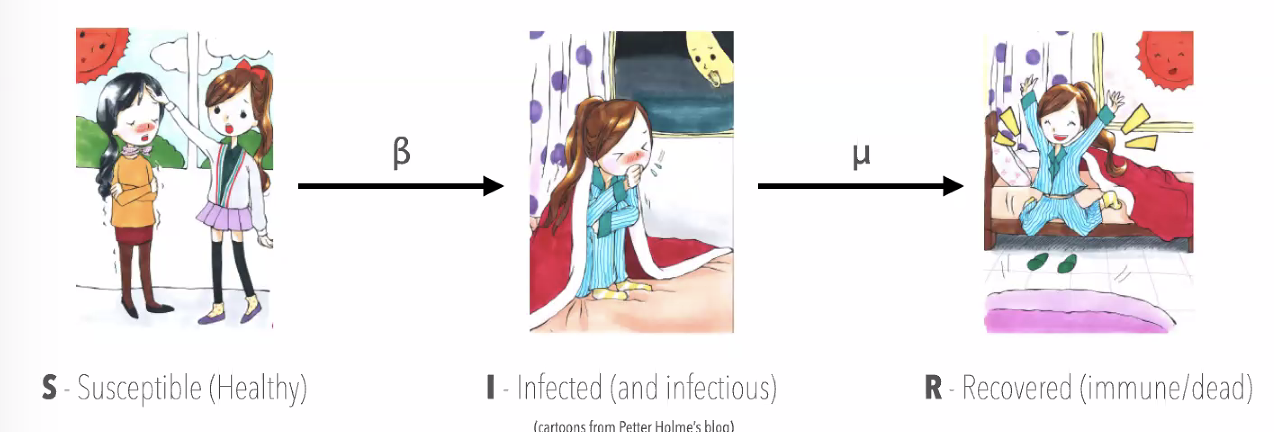
\includegraphics[width=0.9\textwidth]{../lessons/image/02/1_classification.png}
\caption{\label{fig:1_classification} Classification of infected population in three different stages of the disease.}
\end{figure}

Let us consider a population of individuals and try to characterize it. Note as we have not made any assumption on the individuals and relationships between them. We now introduce three different \textbf{compartments}, denoted with \textbf{S} (that stands for \textit{Susceptible}), \textbf{I} (\textit{Infected}), \textbf{R} (\textit{Recovered}), and want to label people according to the stage of their disease, as seen in Fig. \ref{fig:1_classification}. However, one should note that there can be also transitions from one state to another one, according to some rates that describe the \textbf{dynamic}. For instance, in Fig. \ref{fig:1_classification} these are $\beta$ and $\mu$.

This approximation, on the other hand, is quite strong: by keeping the rates fixed we are assuming that the process underlying the spreading of the disease is \textbf{Markovian}. In reality, we do not see exponential distributions (i.e. decays), but some other distributions such as the $Gamma$ one. This last point, however, will be discussed during the course when we will deal with \textbf{“non-Markovian”} epidemics. The interpretation we may give to $\beta$ is the \textit{“per contact” infectious rate}, in this way we only need to count the number of contacts.
Different models can be introduced according to the type of the disease: for instance \textbf{SI}, \textbf{SIR}, \textbf{SIS}, \textbf{SEIR} and so forth.


One should note that medical status is actually different from infectious status. In the latter we do not care about medical status of the person, but only about the disease and how the immune system reacts against it.

As an example, for the \textbf{SEIR} compartmental model, we have four main stages of the disease: starting from a healthy state (\textbf{S}\textit{usceptible}), the individual can contract the disease (\textbf{E}\textit{xposed}) and then, only after some time, becomes infectious (\textbf{I}\textit{nfectious}) until he recovers (\textbf{R}\textit{ecovered}) (Fig. \ref{fig:2_5}). The most important thing to keep in mind is that these compartments are not the same ones of the medical status, since they keep into account different parameters despite the disease is the same one.

\begin{figure}[h!]
\centering
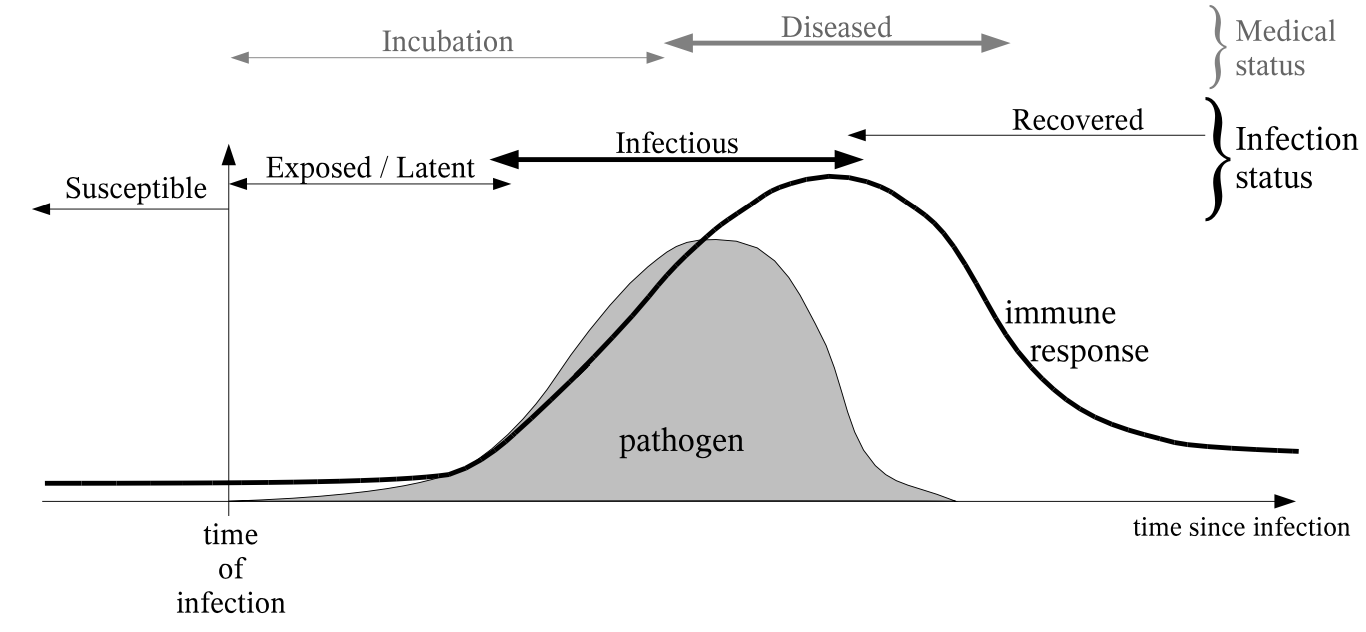
\includegraphics[width=0.7\textwidth]{../lessons/image/02/5.png}
\caption{\label{fig:2_5} A sketch of the time-line of infection, showing the dynamics of the pathogen (grey area) and the host immune response (black line) with the labeling for the various infection classes: \textbf{S}usceptible, \textbf{E}xposed, \textbf{I}nfectious, and \textbf{R}ecovered. Note that the period when symptoms are experienced (medical status) is not necessarily correlated with any particular class of epidemiological models.}
\end{figure}

Now, let us introduce the \textbf{Basic Reproductive Number} $\mathbf{R_0}$ (pr. \textit{"R naught"}) which is a measure of the infection in the population. If we wanted to empirically determine it: we put one guy inside a group for an arbitrarily long time period and, at the end, we count the number of secondary cases that we have. This is the main idea behind the computation of \( R_0 \). This parameters therefore determines whether a disease will spread or not:
  \begin{equation}
    \begin{cases}
     R_0 < 1\\
     R_0 = 1\\
     R_0 > 1\\
    \end{cases}
  \end{equation}
Let us consider the plot of Fig. \ref{fig:2_R_0.png}, we have a sort of \textbf{second order phase transition} at the point $R_0=1$.
Note that $R_0$ for the SARS is higher than the one of COVID-19. However, we did not experienced an outbreak of this disease, so that is not the only parameters to be taken into account in the models. In order to compute $R_0$ we assume that the population is totally susceptible. This is however valid only at the very early stages, later on, we must consider both epidemiological and demographical aspects. The conclusion is the following: $R_0$ may vary from one population to another.

Since we are doing a \textbf{coarse-graining} of the dynamics, this number represents the average of all possible different distributions. A \textit{wrong} argument is to think that similar $R_0$'s lead to similar outbreaks. The distribution of infections can be quite heterogeneous: the mean could be quite representative only if we are dealing with homogeneous populations, that is not the case for real networks. For instance, let us consider the plot in Fig. \ref{fig:3_outbreaks}. We see that SARS was heterogeneous, while Spanish Flu was a more homogeneous one. COVID-19 is most likely somewhere in the middle.

Let us now introduce the \textbf{Effective Reproductive Number} \pmb{R(t)}, which is the same of $R_0$ but varying wrt time. Hence, it is the average number of secondary cases that a single case produces in a population at time $t$.

\begin{figure}[h!]
\centering
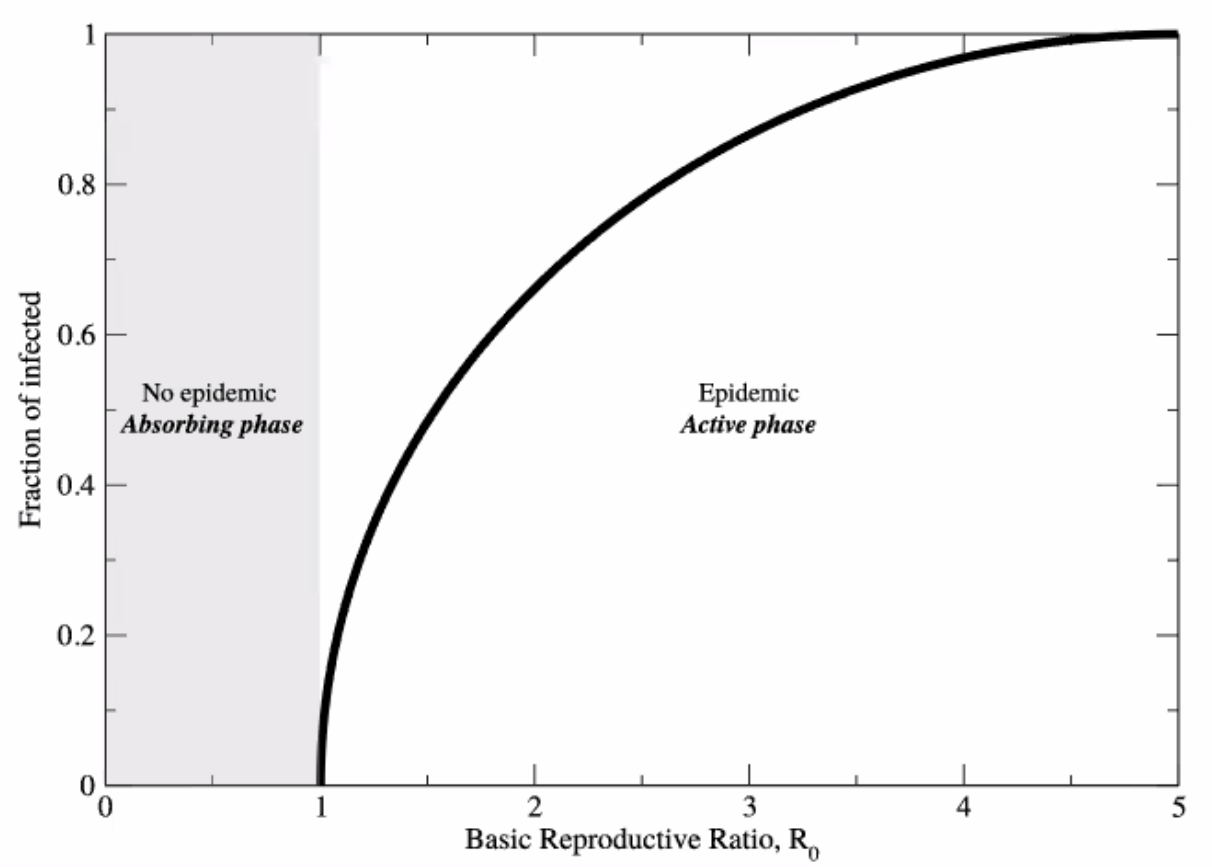
\includegraphics[width=0.7\textwidth]{../lessons/image/02/2_R_0.png}
\caption{\label{fig:2_R_0.png} Fraction of infected vs basic Reproductive Ratio, \( R_0 \).}
\end{figure}

\begin{figure}[h!]
\centering
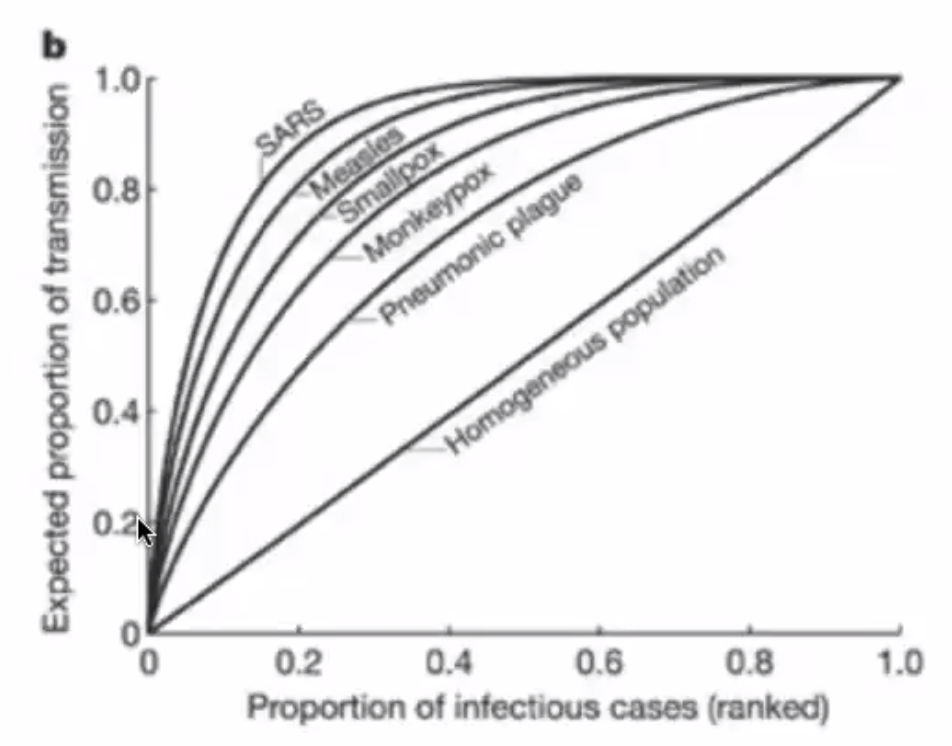
\includegraphics[width=0.6\textwidth]{../lessons/image/02/3_outbreaks.png}
\caption{\label{fig:3_outbreaks} Figure from: Lloyd-Smith et al. Nature 438, 355–359 (2005).}
\end{figure}

\begin{figure}[h!]
\centering
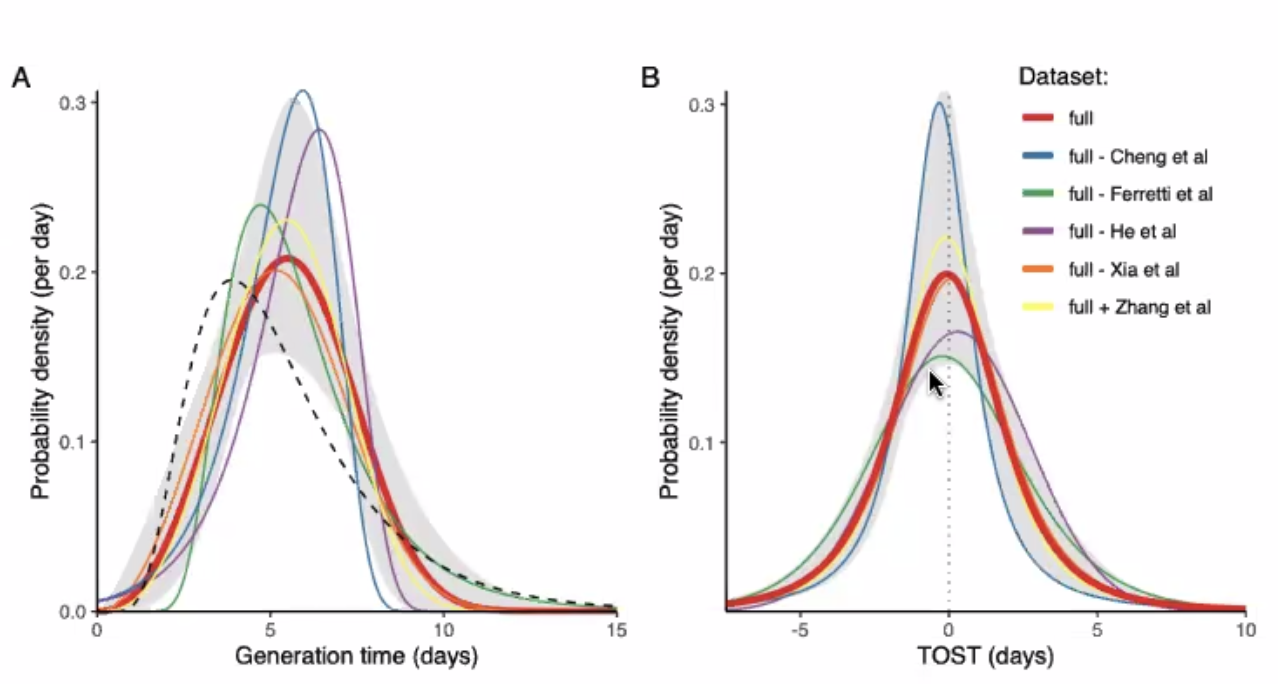
\includegraphics[width=0.6\textwidth]{../lessons/image/02/4_TOST.png}
\caption{\label{fig:4_TOST} Figure from: Ferretti et al. \url{https://www.medrxiv.org/content/10.1101/2020.09.04.20188516v1}}
\end{figure}



Other important quantities we may want to introduce are:

\begin{itemize}
    \item \textbf{Infectious period}: average period for a person to be infectious is computed either as $ \tau = \frac{1}{\mu }$ or $\quad \tau = \frac{1}{(\alpha + \mu )} $ where the presence of $\alpha$ depends on the model ($\alpha$: average duration of "exposed time" stay).
    \item \textbf{Incubation period}: period of time between infection to occurrence of symptoms
    \item \textbf{Generation time}: time for an infected person to generate a second infection
    \item \textbf{Serial interval}: time between the onset of symptoms for a person and the onset of symptoms for another second infected person
    \item \textbf{TOST}: time between the onset of symptoms to an infection
    
\end{itemize}
A problem in predicting a possible outbreak of a disease is that TOST in many cases can be negative (see Fig. \ref{fig:4_TOST} for more details).










\end{document}
